
\chapter{解决方案}
\label{chap:contribute}

在这个网络如此发达,web2.0和云计算的使用日益普及的时代,人们的文档管理方式也发生了巨大的改变。但是由于种种原因,有些好的模式和方法并没有被高校用户所认可与广泛使用。而且可以证实,有些公共网络上的文档服务也并不适合高校用户。所以就导致了大部分高校用户的个人文档管理方式依然停留在10年前的单机模式下,也就势必带来本文上一章所提到的诸多文档管理的问题。而本文描述系统的设计目标就是帮助高校用户解决这些问题。本章下面就针对上面提到的每一个问题逐一提出本系统的解决方案。

\section{文档写作解决方案}
\label{sec:write}

\subsection{LaTex}
\label{sec:latex}

上一章提到,高校用户文档写作过于依赖Word软件,带来的诸多弊端。但是,在很多人看来Word依然是用来写文档的绝佳选择。在我国,Word的普及率如此之高,它有的时候甚至会被认为是编辑文档的唯一选择。仅“所见即所得”一项,Word就会赢得绝大多数用户的心。但是很多人也许不知道,在国外,对于写学术报告和科技论文,有更加标准也更加普及的编辑工具,那就是\LaTeX,世界上很多著名的出版机构斗接受或强制要求作者使用\LaTeX稿件,接受 LaTeX 稿件的出版社大都有自己的文稿样式模板,主要就是一个类型文件包,简称类包。如果稿件未被甲出版社采用,在转投乙出版社前,只需将稿件第一句中类包名称由甲出版社的改为乙出版社的,整篇稿件的样式就随之自动转换过来了,确实很方便。国外知名大学也大多都要求学生使用\LaTeX编写科技报告和论文,这和国内Word一家独大的局面截然不同。本系统用来解决文档编辑问题的基础之一就是\LaTeX。那么什么是\LaTeX呢?

\LaTeX是一种排版系统,它基于\TeX\footnote{国计算机教授高德纳在1978年编写的功能强大的排版软件,高德纳最早开始自行编写它的原因是当时十分粗糙的排版水平已经影响到他的巨著《计算机程序设计艺术》(The Art of Computer Programming)的印刷质量。他以典型的黑客思维模式,最终决定自行编写一个排版软件。}排版系统并由此发展而来。它是由美国电脑学家莱斯利·兰伯特在20世纪80年代初期开发,利用这种格式,即使用户没有排版和程序设计的知识也可以充分发挥由\TeX所提供的强大功能,能在几天,甚至几小时内生成很多具有书籍品质的印刷品。对于生成复杂表格和数学公式,这一点表现得尤为突出。因此它非常适用于生成高印刷质量的科技和数学类文档。这个系统同样适用于生成从简单的信件到完整书籍的所有其他种类的文档。与其他的文字排版系统(比如Word)相比,\LaTeX最突出的优势就是高质量、高专业水准的文稿排版效果。下面简单比较一下\LaTeX和Word:
\begin{description}
\item[入门难度]  Word 特点就是“所见即所得”,其基本功能初学者很容易掌握,很多 Word 用户都是无师自通。但随着篇幅和复杂程度的增加,花费在文稿格式上的精力和时间要明显加大,如图~\ref{fig:xfig2}蓝色示意曲线所示。因为创建自定义编号、交叉引用、索引和参考文献等就不是“所见即所得”了,得耐着性子反复查阅 Word 的在线帮助或借助相关软件帮忙。
对于 \LaTeX 初学者,即就是编排很简单的文章,也要花较多的精力和时间去学习那些枯燥的命令和语法,特别是排写数学公式,经常出错,多次编译不能通过,使很多初学者望而却步。可是一旦掌握,不论文 稿长短和复杂与否都会熟练迅速地完成,先前学习 \LaTeX 的精力投入将由此得到回报,如图~\ref{fig:xfig2}红色示意曲线所示。
\begin{figure}[H]
  \centering
  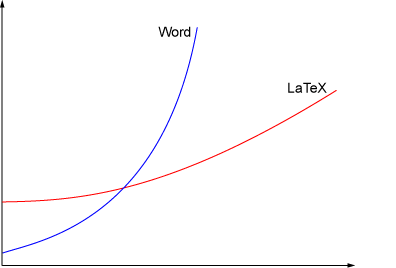
\includegraphics{latexVSword}
  \caption{latex与word的学习曲线比较}
  \label{fig:xfig2}
\end{figure}
\end{description}







\section{文档存储解决方案}
\label{sec:save}

\section{文档分发解决方案}
\label{sec:giveout}

\section{个人成果展示方案}
\label{sec:display}

\section{项目管理解决方案}
\label{sec:project}




